\section{Design}
\label{sec:design}

The standard web login protocol requires the user to input their cleartext password and transmit it to the server, ideally via HTTPS. The WATSUP protocol derives a pseudorandom number generator (PRNG) seed from a key derivation function a user's base password with the hostname and username as a salt. While salting the hostname protects the user against password reuse, salting the username protects against poor server-side salting and hashing. The PRNG is used to generate an asymmetric key pair, which is used to prove identity by decrypting a server-generated nonce.

\begin{figure}
    \centerline{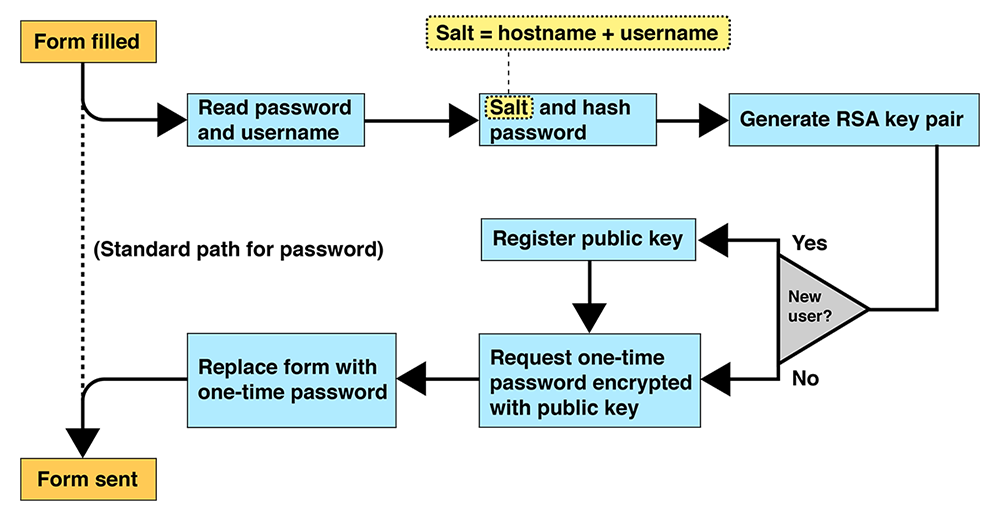
\includegraphics{protocol.png}}
    \caption{Protocol control flow}
\end{figure}

WATSUP generates a unique asymmetric key pair for each site. The key pair is generated with:

\begin{verbatim}
salt = SHA_256(SHA_256(hostname)
               | SHA_256(username))
bits[256] = PBKDF2(root_pass, salt,
                   1000, SHA_256)
prng = seed_ARC4(bits)
key_pair = rsa_key_gen(prng)
\end{verbatim}

Upon registration, the user's public key is stored on the web server. When the user logs in, the server sends the user a cryptographic nonce, encrypted with the user's public key. The WATSUP client uses the generated private key to decrypt the nonce, which it sends to the server as proof of identity.

To support the WATSUP protocol, a server needs to implement the following specifications:

\begin{itemize}

    \item On registration, the server stores the username and associated public key.

    \item On OTP request, generate a cryptographic nonce, associate the nonce with the requesting username, fetch the user's public key, use RSA to encrypt the nonce with the public key, and return the encrypted nonce.

    \item On authentication request, verify the received nonce matches the known nonce. If they match, mark the user as logged in. If not, reject the request.

\end{itemize}




